% Author: Till Tantau
% Source: The PGF/TikZ manual
\documentclass{article}

\usepackage{tikz}
\usepackage{verbatim}

\begin{document}
\pagestyle{empty}

\begin{comment}
:Title: Automata
:Tags: Manual, Automata, Foreach, Graphs

This example is from the System layer  title page of the TikZ and PGF manual.

| Author: Till Tantau
| Source: The PGF/TikZ manual

\end{comment}
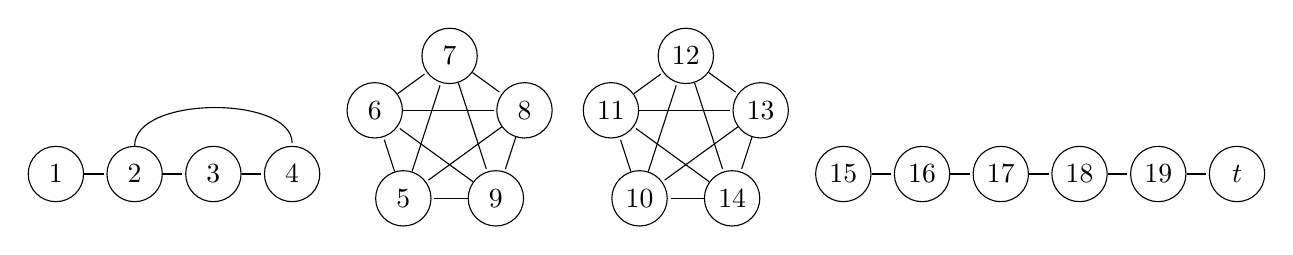
\begin{tikzpicture}[shorten >=1pt,-]
  \tikzstyle{vertex}=[circle,draw=black,fill=white!25,minimum size=20pt,inner sep=0pt]

  \foreach \name/\x in {1/1, 2/2, 3/3, 4/4, 15/11, 
                        16/12, 17/13, 18/14, 19/15, t/16}
    \node[vertex] (G-\name) at (\x,0) {$\name$};

  \foreach \name/\angle/\text in {P-1/234/5, P-2/162/6, 
                                  P-3/90/7, P-4/18/8, P-5/-54/9}
    \node[vertex,xshift=6cm,yshift=.5cm] (\name) at (\angle:1cm) {$\text$};

  \foreach \name/\angle/\text in {Q-1/234/10, Q-2/162/11, 
                                  Q-3/90/12, Q-4/18/13, Q-5/-54/14}
    \node[vertex,xshift=9cm,yshift=.5cm] (\name) at (\angle:1cm) {$\text$};

  \foreach \from/\to in {1/2,2/3,3/4,3/4,15/16,16/17,17/18,18/19,19/t}
    \draw (G-\from) -- (G-\to);

  \foreach \from/\to in {1/2,2/3,3/4,4/5,5/1,1/3,2/4,3/5,4/1,5/2}
    { \draw (P-\from) -- (P-\to); \draw (Q-\from) -- (Q-\to); }

    % \draw (G-2) .. controls (2,-1) and (4,-1) .. (G-4);
    \draw (G-2) .. controls (2, 1) and (4, 1) .. (G-4);
%   \draw (G-3) .. controls +(-30:2cm) and +(-150:1cm) .. (Q-1);
%   \draw (Q-5) -- (G-15);
  
\end{tikzpicture}

\end{document}